\documentclass[a4paper]{bxjsarticle}

\usepackage{luatexja}
\usepackage{luacode}
\usepackage{graphicx}

\usepackage{enumitem}

\usepackage{adjustbox}
\usepackage{amsmath, amssymb}

\setpagelayout*{margin=20truemm}

% タイトルを調節
\makeatletter
\def\@maketitle{%
	\newpage\null
	\begin{center}%
		\let\footnote\thanks
		{\Large \@title \par}%
		\ifx\bxjs@subtitle\@undefined\else
			\vskip3\p@?
			{\normalsize \bxjs@subtitle\par}
		\fi
		\vskip 1em
		{\large
			\lineskip .5em
			\begin{tabular}[t]{c}%
				\@author
			\end{tabular}\par}%
		\vskip 1em
		{\large \@date}%
	\end{center}%
	\par\vskip 1.5em
	\ifvoid\@abstractbox\else\centerline{\box\@abstractbox}\vskip1.5em\fi
}
\makeatother

% 論理式を簡単に記述できるようにする
\begin{luacode*}
  function boolex(expr)
    expr = string.gsub(expr, "*", [[\cdot ]])
    expr = string.gsub(expr, "><", [[>\,<]])
    expr = string.gsub(expr, "<", [[\overline{]])
    expr = string.gsub(expr, ">", [[}]])
    expr = string.gsub(expr, "@", [[\oplus ]])
    expr = string.gsub(expr, "-", [[\downarrow ]])
    return expr
  end
\end{luacode*}

\newcommand{\boolex}[1]{\directlua{tex.sprint(boolex("#1"))}}


\title{2021年度 論理設計 レポート課題}
\author{\directlua{tex.print(os.getenv("AUTHOR_NAME"))}}
\date{提出日:2022年01月22日}


\begin{document}
  \maketitle

  \section*{問2.10}
  $$f=\boolex{A<B>+<A>(B+<C>)}$$
  をNAND形式,NOR形式にそれぞれ変換後,論理回路で実現しなさい.
  \begin{align*}
    f
    &=\boolex{<<A*<B>+<A>*(B+<C>)>>} \\
    &=\boolex{<<A*<B>>*<<A>*(B+<C>)>>} \\
    &=\boolex{<<A*<B>>*<<A>*<<B+<C>>>>>} \\
    &=\boolex{<<A*<B>>*<<A>*<<B>*C>>>} \\
    &=\boolex{<<A*<B*B>>*<<A*A>*<<B*B>*C>>>} &\text{(NAND形式)} \\
  \end{align*}
  \begin{center}
    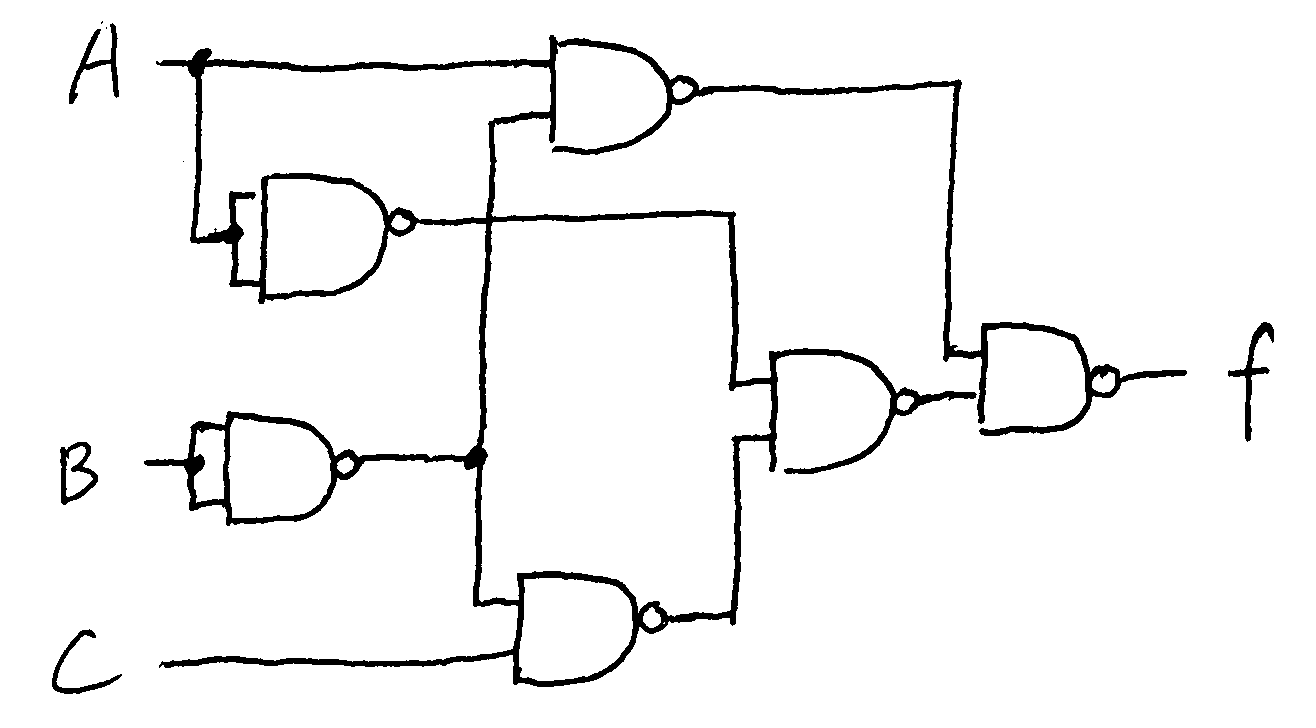
\includegraphics{1-a.png}
  \end{center}
  \begin{align*}
    \boolex{<f>}
    &=\boolex{<A<B>>*<<A>(B+<C>)>} \\
    &=\boolex{(<A>+B)*(A+<(B+<C>)>)} \\
    f
    &=\boolex{<<A>+B>+<A+<B+<C>>>} \\
    &=\boolex{<<A+A>+B>+<A+<B+<C+C>>>} \\
    &=\boolex{<f_1+f_1>},\qquad\boolex{f_1=<<<A+A>+B>+<A+<B+<C+C>>>>} &\text{(NOR形式)} \\
  \end{align*}
  \begin{center}
    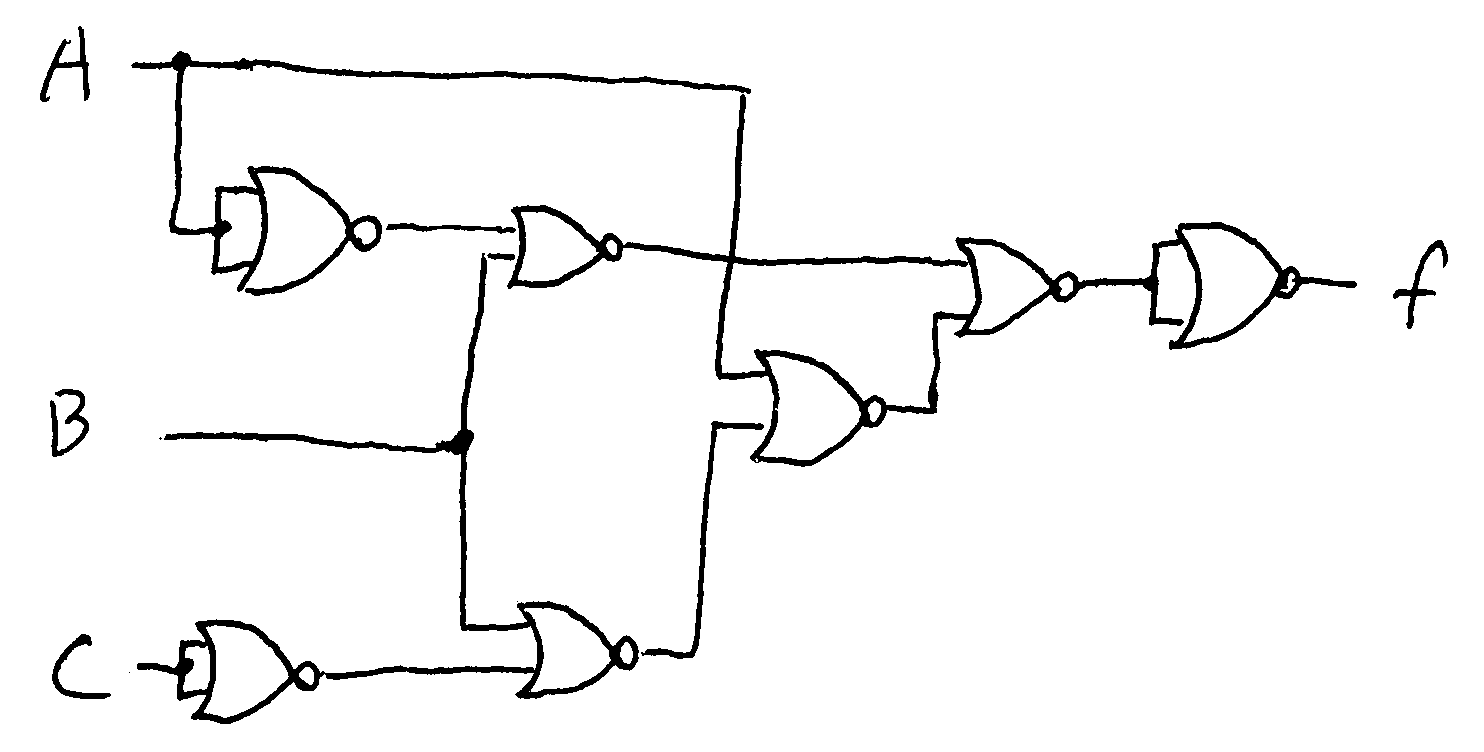
\includegraphics{1-b.png}
  \end{center}

  \section*{問3.1}
  次の論理式をブール代数の公理を用いて簡単化しなさい.
  \begin{enumerate}[label=(\arabic*)]
    \item $f=\boolex{A*<B>+<A>*<B>}$
      $$f=\boolex{(A+<A>)*<B>}=\boolex{1*<B>}=\boolex{<B>}$$
    \item $f=\boolex{A*B+<A>*B+A*<B>}$
      $$f=\boolex{(A+<A>)*B+A*<B>}=\boolex{B+A*<B>}=\boolex{(B+A)*(B+<B>)}=\boolex{B+A}$$
  \end{enumerate}

  \section*{問3.2}
  次の論理関数を簡単化し,論理回路を描きなさい.また,真理値表を作成し,
  論理関数の簡単化前後で論理が合っているか確認しなさい.
  \begin{enumerate}[label=(\arabic*)]
    \item $f=\boolex{A*B+<A>*B+<A>*<B>}$
      $$
      f
      =\boolex{(A+<A>)*B+<A>*<B>}
      =\boolex{B+<A>*<B>}
      =\boolex{(B+<A>)*(B+<B>)}
      =\boolex{<A>+B}
      $$
      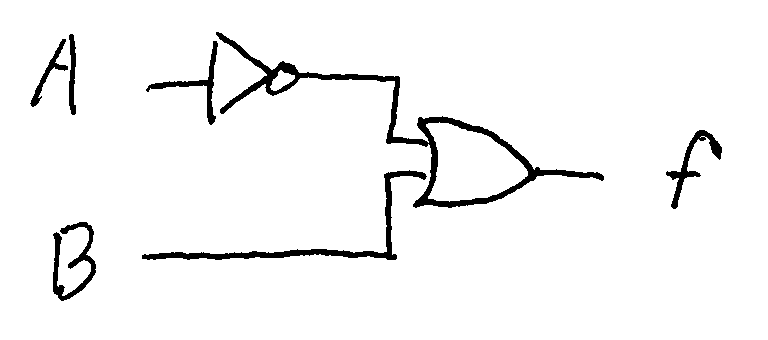
\includegraphics{3-1.png}
      \begin{minipage}{10cm}
        $$
        \begin{array}{ccc|cccc|c}
          A&B&C & \boolex{A*B}&\boolex{<A>*B}&\boolex{<A>*<B>}&f & \boolex{<A>+B} \\ \hline
          0&0&0 & 0&0&1&1 & 1 \\
          0&0&1 & 0&0&1&1 & 1 \\
          0&1&0 & 0&1&0&1 & 1 \\
          0&1&1 & 0&1&0&1 & 1 \\
          1&0&0 & 0&0&0&0 & 0 \\
          1&0&1 & 0&0&0&0 & 0 \\
          1&1&0 & 1&0&0&1 & 1 \\
          1&1&1 & 1&0&0&1 & 1
        \end{array}
        $$
      \end{minipage}
    \item $f=\boolex{A*(B*C+<B>*C)}$
      $$
      f
      =\boolex{A*((B+<B>)*C)}
      =\boolex{A*C}
      $$
      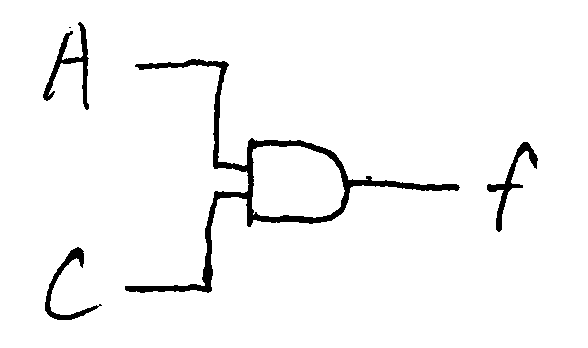
\includegraphics{3-2.png}
      \begin{minipage}{10cm}
        $$
        \begin{array}{ccc|cc|c}
          A&B&C & \boolex{B*C+<B>*C}&f & \boolex{A*C} \\ \hline
          0&0&0 & 0&0 & 0 \\
          0&0&1 & 1&0 & 0 \\
          0&1&0 & 0&0 & 0 \\
          0&1&1 & 1&0 & 0 \\
          1&0&0 & 0&0 & 0 \\
          1&0&1 & 1&1 & 1 \\
          1&1&0 & 0&0 & 0 \\
          1&1&1 & 1&1 & 1
        \end{array}
        $$
      \end{minipage}
    \item $f=\boolex{A+A*B+<A>*B}$
      $$
      f
      =\boolex{A+(A+<A>)*B}
      =\boolex{A+B}
      $$
      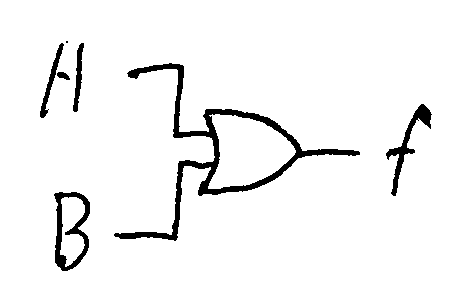
\includegraphics{3-3.png}
      \begin{minipage}{10cm}
        $$
        \begin{array}{cc|c|c}
          A&B & f & \boolex{A+B} \\ \hline
          0&0 & 0 & 0 \\
          0&1 & 1 & 1 \\
          1&0 & 1 & 1 \\
          1&1 & 1 & 1
        \end{array}
        $$
      \end{minipage}
    \newpage
    \item $f=\boolex{A*B*C+A*C+A*B*<C>}$
      $$
      f
      =\boolex{A*B*(C+<C>)+A*C}
      =\boolex{A*B+A*C}
      =\boolex{A*(B+C)}
      $$
      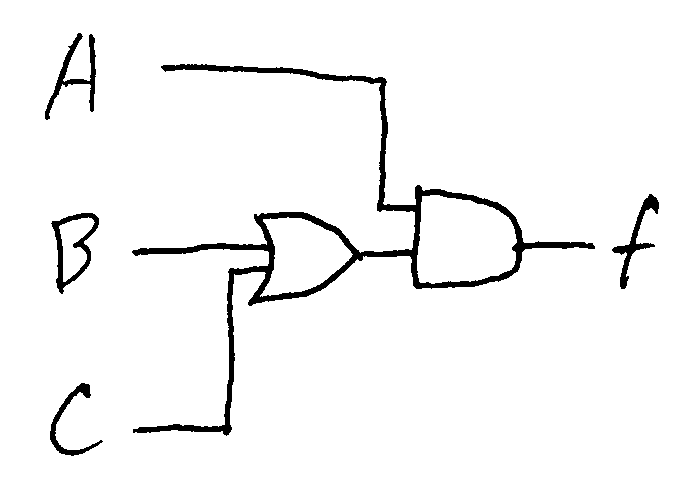
\includegraphics{3-4.png}
      \begin{minipage}{10cm}
        $$
        \begin{array}{ccc|c|c}
          A&B&C & f & \boolex{A*(B+C)} \\ \hline
          0&0&0 & 0 & 0 \\
          0&0&1 & 0 & 0 \\
          0&1&0 & 0 & 0 \\
          0&1&1 & 0 & 0 \\
          1&0&0 & 0 & 0 \\
          1&0&1 & 1 & 1 \\
          1&1&0 & 1 & 1 \\
          1&1&1 & 1 & 1
        \end{array}
        $$
      \end{minipage}
  \end{enumerate}
\end{document}